\chapter{Design} \label{chp:design}

\section{Introduction}
This chapter will go through the design of a \program{Publisher} and \program{Subcriber} that fulfils the requirements listed in table \ref{tab:requirements}.
At first, this chapter will go through the \textit{Design Requirements} in section \ref{sec:design:requirements} which list the design principles used in this chapter.
In section \ref{sec:design:vcs} a \ac{VCS} is explained, as a \ac{VCS} has similar functionality, as described in section~\ref{sec:streamingidea}.
From the \ac{VCS}, the most widely-used protocols are explained in sections \cref{test, test1, test2}.
At last, the protocols are compared to the requirements from section \ref{sec:analysis:requirements}, in order to find the most suitable protocols.
This chapter will then end up with a list of design choices and requirements for the implementation.

\section{Design Requirements} \label{sec:design:requirements}
The proposed system is designed with the concepts of the UNIX philosophy in mind:
\begin{itemize}
	\item Programs should do one thing, and do it well.
	\item Programs should be able to work together.
	\item Programs should be capable of taking streams (of text) as input.
\end{itemize}

\todo{"always use the simplest solution possible" (Rich, 1995, pp. 221 and 231) and McIlroy
recommends (slightly modified) "creating components that do one thing and do it well"}

By complying with the three ideas from above, the system should consist of multiple small programs that can be put together in different ways to serve different purposes.

Since the system is developed for biologists, it should be easy to use and require minimum intervention to get it running. Ideally the system should be “plug and play” such that biologists can take the number of recording boxes required for their application and put it all together without the need to configure software on any of the boxes. \todo{Add Extensibility somewhere, maybe not due to maintainability}

\todo{Add: Write as little code as possible, use already existing code maintained by other developers}
\todo{add: Should be a requirement that it should be easy to write new nodes. Should not require an interface to send commands, should be self-contained as possible.}

\todo{Design inspired by Daniel J. Bernstein, software run in "chains"}
Furthermore the system should also be:

\begin{itemize}
	\item Maintainable:
As other people will improve the system in the future, it should also be easy to maintain. This will almost happen automatically if the ``UNIS design rules'' are kept in mind during design and development.
\item Modular:
The system should consist of multiple small programs which can be used in all existing use-cases but also those that might come in the future.
\item Reusable:
As much code should be as reusable as possible in order to avoid implementing the same functionality multiple times.
\item Extensible
    By implementing small programs, the system should be easy to extend in the future.
    If functionality is missing in one of the programs, it should be possible to create a new 
    program with the new functionality.
\end{itemize}

However splitting functionality into multiple modules will also be done with caution as it might come with the price of performance. Each time programs are split up, there is usually required some communication between the programs or some exchange of memory. The communication might turn out to be unnecessary performance consumption. Therefore splitting programs up is seen as simplicity(as it eases development and use) vs. performance.

\todo{a trade-off between simplicity vs. performance}

\section{Video conference System(VCS)}
% http://www.faqs.org/rfcs/rfc5219.html <- mp3 i rtp
% RTP description https://flylib.com/books/en/4.245.1.27/1/
\ac{VCS} utilize audio and video streams, as a video conference is a connection between people residing in separate locations. This connection gives the impression that people participating in the video conference are present in the physical meeting. VCS usually allows for multiple participants to join a meeting where all participants are able to see each other. VCS might allow control of the camera by the remote participant in order to look at the person who is currently speaking. 
Lip-sync is often preferred during the video conference, to further give the impression the remote-participant is present. Lip-sync is when the sound from the remote participants is synchronized with the video stream. This usually has to be implemented by the streaming protocols as sound and video is not necessarily transmitted in the same stream and so are not synchronized when received by the recipient.

\begin{figure}[H]
	\centering
	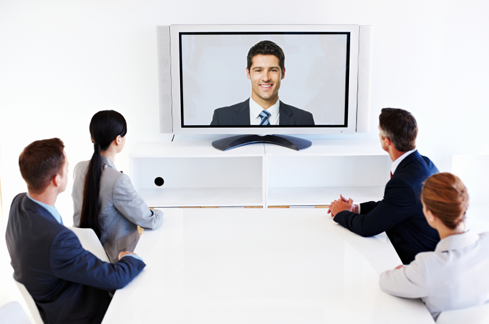
\includegraphics[width=0.8\textwidth]{figures/vcs_overview.png}
	\caption{Example of a video conference system where five people are participating in a meeting, but the third person is not physically present.} \label{fig:design:vcs}
\end{figure}

\ac{VCS} works similarly to \ac{VoIP}, which is like a conference system between two participants only using sound. A typical protocol stack is shown in figure~\ref{fig:design:protocolstack}. 

%rtcp used to adjust codec wrt. bandwidth
\begin{figure}[H]
	\centering
	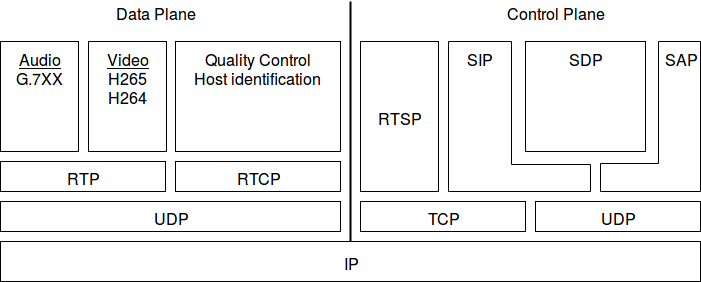
\includegraphics[width=\textwidth]{figures/protocol_stack}
	\caption{Protocols used in VCS and VoIP. It should be noted, that not all protocols necessarily are used at the same time.}
	\label{fig:design:protocolstack}
\end{figure} 

\todo{Citation for figure?}

Figure \ref{fig:design:protocolstack} shows how the protocols stack on top of each other, where IP is in the bottom layer in the \textit{Data Plane} and \textit{Control Plane}. The  \textit{Data Plane} is where the encoded audio and video is transferred, between participating nodes. Part of the \textit{Data Plane} is also the RTCP protcol, which provides channel information about the quality between participants. Usually the RTP protocol is used to packetize encoded audio and video - encoding is handled by G.7XX or H264/H265. The \textit{Control Plane} is where sessions are initiated. In VoIP, SIP is usually used to initiate sessions, but other protocols such as RTSP and SAP can be used as well. Which protocol is used to initiate the session depends on the application and whether it is a session between multicast participants or unicast. SDP is used in SIP to negotiate supported codecs between participants\todo{Between sender and receiver}, but used in RTSP and SAP to describe a session with encoding statically set by the session originator\citep{voip_fundamentals}

The protocols in figure \ref{fig:design:protocolstack} are listed in table~\ref{tab:design:protocollist}. Proprietary VCSs such as Skype use closed protocol specifications which are not included in the table.


\begin{table}[H]
	\centering
	\resizebox{\textwidth}{!}{%
		\begin{tabular}{@{}|l|l|l|l|@{}}
			\toprule
			\textbf{Protocol}              & \textbf{Described in} & \textbf{Functionality} \\ \midrule
			Real time Transport Protocol (RTP)    & \ref{sec:design:rtp}                  & Transports video, sound etc.\\ \midrule
			Real time Control Protocol (RTCP)          & \ref{sec:design:rtcp}                & Quality feedback, participant ident. and timing\\ \midrule
			Session Description Protocol (SDP)   & \ref{sec:design:sdp}                  & Describes a RTP session\\ \midrule
			Session Announcement Protocol (SAP)  & \ref{sec:design:sap}                  & Announces a SDP on multicast group\\ \midrule
			Real Time Streaming Protocol (RTSP) & \ref{sec:design:rtsp} & Creates session \\ \bottomrule
		\end{tabular}%
	}
	\caption{Table shows protocols often used in video conference systems}
	\label{tab:design:protocollist} 
\end{table}
\todo{Add RFC to table for each protocol}

\todo{Add RTSP and other non-relevant protocols?}

\section{Real-time Transport Protocol} \label{sec:design:rtp}
The RTP protocol is a network protocol for transmitting media such as audio, video and text in streaming applications such as \ac{VoIP} and video conference systems. The terminology used throughout the thesis is from RFC7656\citep{RFC7656}. Not all terms defined in RFC7656 are used in attempt to limited the scope of the RTP terminology used in this thesis. Details are the RTP protocol is from RFC3550\citep{RFC3550}.

The RTP protocol does not specify how the data should be packet into the payload of an RTP packet. This is defined by profiles and packet types. A profile can contain multiple data formats, and might describe some general details about the content of the RTP packet.
The most used profile is the ``RTP/AV audio video for conference with minimal control'', which is used for streaming audio and video witch is described in section \ref{sec:design:profile}.

\myparagraph{RTP Stream} \label{sec:design:rtpstream}
RTP packets are sent in RTP streams. An RTP stream corresponds to a source stream as introduced in section \ref{sec:analysis:pubsub}. RTP is usually run over UDP, but it can be used over TCP as well. RTP is typically used with port 5004, but 5004 is not assigned to RTP by IANA\citep{iana_ports}.


\myparagraph{RTP Session} \label{sec:design:rtpsession}
An RTP Session is a group of participants communication using RTP.
An RTP stream is sent in a RTP session, such that participants in that session receive the RTP stream. An RTP session can potentially carry multiple RTP streams. Within an RTP session, every participant can find metadata and control information (over RTCP) about all the RTP streams in the RTP session. A participant can be involved in multiple RTP sessions e.g. when a participant receive more than one media. In RTP sessions, each media is typically carried in a separate RTP session with its own RTCP packets unless the the encoding itself multiplexes multiple media into a single data stream. See RTCP packets in section \ref{sec:design:rtcp}. Multiple RTP sessions are usually referred to as a multimedia session.


An RTP session can be identified in two ways:
\begin{itemize}
	\item In unicast with e.g. two participants talking to each other, an RTP session is defined as two destination transport addresses, each with a port pair for RTP and RTCP. This allows both participants to send RTP and RTCP packets to each other.
	\item In multicast with N participants, an RTP session is defined as a destination transport address and a port pair. This allows multiple participants to send and receive RTP streams by sending and receiving from the multicast address.
\end{itemize}

\myparagraph{RTP Packet}
An RTP packet is depicted in figure~\ref{fig:design:rtppacket}. The static RTP header is 12 bytes, when no CSRC is present and no additional headers.
\todo{Describe CSRC + header extensions}

\begin{figure}[H]
\centering
\begin{verbatim}
    0                   1                   2                   3
    0 1 2 3 4 5 6 7 8 9 0 1 2 3 4 5 6 7 8 9 0 1 2 3 4 5 6 7 8 9 0 1
   +-+-+-+-+-+-+-+-+-+-+-+-+-+-+-+-+-+-+-+-+-+-+-+-+-+-+-+-+-+-+-+-+
   |V=2|P|X|  CC   |M|     PT      |       sequence number         |
   +-+-+-+-+-+-+-+-+-+-+-+-+-+-+-+-+-+-+-+-+-+-+-+-+-+-+-+-+-+-+-+-+
   |                           timestamp                           |
   +-+-+-+-+-+-+-+-+-+-+-+-+-+-+-+-+-+-+-+-+-+-+-+-+-+-+-+-+-+-+-+-+
   |           synchronization source (SSRC) identifier            |
   +=+=+=+=+=+=+=+=+=+=+=+=+=+=+=+=+=+=+=+=+=+=+=+=+=+=+=+=+=+=+=+=+
   |            contributing source (CSRC) identifiers             |
   |                             ....                              |
   +-+-+-+-+-+-+-+-+-+-+-+-+-+-+-+-+-+-+-+-+-+-+-+-+-+-+-+-+-+-+-+-+
   |                             Payload                           |
   |                              ....                             |
   |                              ....                             |
   +-+-+-+-+-+-+-+-+-+-+-+-+-+-+-+-+-+-+-+-+-+-+-+-+-+-+-+-+-+-+-+-+
\end{verbatim}
\caption{Figure of how the RTP packet is structured\citep{RFC3550}}
\label{fig:design:rtppacket}
\end{figure}

\myparagraph{Payload}
\myparagraph{SSRC}
The \ac{SSRC} field is a 32 bits identifier that uniquely identifies a participant within an RTP session. All RTP and RTCP packets sent by a participant carries the same SSRC, such that receiving participants know where a RTP or RTCP packet belongs to. In case a property of a RTP stream such as encoding, the SSRC must change such that receiving participants is aware of the property change.

\myparagraph{Timestamp}
The timestamp is a 32 bit NTP timestamp with random offset that reflects the sampling instant of the first octet in the RTP packet. Multiple consequence, logically generated at once, RTP packets can have the same timestamp, in case the payload of multiple RTP packets are related such as in a video frame.
The timestamp is also used to synchronize multiple RTP streams and to estimate jitter in order to provide quality feedback to the sender using RTCP RR as described in section~\ref{sec:design:rtcp}.
As the clock frequency is dependent on the content of the RTP packet, the clock frequency is specified in the payload specification. This is usually specified in a SDP as described in section~\ref{sec:design:sdp}. As an example, for fixed-rate audio the timestamp clock would likely increment by one for each sampling period. If an audio application reads blocks covering 160 sampling periods from the input device, the timestamp would be increased by 160 for each such block\citep{RFC3550}.

To synchronize a single RTP stream, the timestamp can be used however; if multiple RTP streams should be synchronized e.g. in the case of video and audio, the timestamps are not enough, as they may advance at different speeds with different offsets. The timestamp is then used together with RTCP SR packets, with associates the timestamp with a 64 bit NTP timestamp. The RTCP SR packet is usually sent with a lower frequency than the 32 bit timestamp. The 64 bit reference clock is shared between multiple media streams to be synchronized. The RTCP SR packet is described in section~\ref{sec:design:rtcp}.


\myparagraph{Sequence Number}
The sequence number is a 16 bit integer that can be used by receiving participants to estimate the packet loss. This value must be randomly initialized.

\myparagraph{Payload}
The payload is the content of the RTP packet. This is the encoded media such as audio or video. 

\myparagraph{Packet Type}
The packet type identifies the format of the payload. RFC3550 does not define which values that can be used.


\myparagraph{Mark bit}
The mark bit can be used to signal significant events. RFC3550 does not specify how this bit should be used.

\todo{RTP supports header extentions}


\section{Real-time Control Protocol} \label{sec:design:rtcp}
RTCP provides metainformation about an RTP stream.
Usually port = RTP port +1


RTCP is used to provide reception quality feedback, participant identification, and synchronization between RTP streams.

RTCP carries a persistent transport-level identifier for an RTP
      source called the canonical name or CNAME, Section 6.5.1.  Since
      the SSRC identifier may change if a conflict is discovered or a
      program is restarted, receivers require the CNAME to keep track of
      each participant.  
      
      By having each
      participant send its control packets to all the others, each can
      independently observe the number of participants.

RTCP runs alongside RTP and provides periodic reporting of this information. Although data packets are typically sent every few milliseconds, the control protocol operates on the scale of seconds.

The information sent in RTCP is necessary for synchronization between RTP streams for example, for lip synchronization between RTP streams carrying audio and video and can be useful for adapting the transmission according to reception quality feedback, and for identifying the participants.


- therefore each periodically transmitted compound RTCP
      packet MUST include a report packet.
      
- so each compound RTCP packet MUST also
      include the SDES CNAME
      
      When a participant wishes to leave a session, a BYE packet is
   transmitted to inform the other participants of the event.

\newcommand{\itemmsg}[1]{\item \textbf{#1}}

The RTCP protocol contains the following message types:
\begin{itemize}
	\itemmsg{Sender Report(SR)}
	\itemmsg{Receiver Report(RR)}
	\itemmsg{Source Description(SDES)}
	\itemmsg{Membership Management(BYE)}
	\itemmsg{Application-Defined(app)}
\end{itemize}



\todo{Verify clockrate(timestamp) is in order with RTP packet timestamp description}
\subsection{Profile} \label{sec:design:profile}
RTP leaves out many details about how streams should be send.
Examples of this are listed below:
\begin{itemize}
	\item How encoded media is mapped into the \textit{Packet Type}-field in the RTP header
	\item How often RTCP Sender-Reports and Recever-Reports should be sent.
	\item How audio and video should be packet into a stream e.g. How to know which channel a sample belongs to.
	\item Calculation of the clock rate in \textit{Timestamp}-field.
	\item The semantics of the \textit{Marker}-bit.
\end{itemize}

Profiles answer the questions listed above, and many more details regarding semantics of the RTP packet fields. Generally, the \textit{RTP Profile for Audio and Video Conferenceswith Minimal Control}\citep{RFC3551} profile is used in audio and video systems.\citep{perkins2003rtp}.

The Audio/video specifies different \textit{Payload Formats} that can be used in the RTP stream. Initially the Audio/Video profile should define all encodings available, but later on it was discovered to be easier to reserve a range of dynamic types, such that the profile didn't have to define all possible encodings. If a dynamic type is chosen, the SDP describes the properties of the stream such as encoding, sample size, bitrate, number of channels etc. The SDP is described in section \ref{sec:design:sdp}.

The \textit{Marker}-bit is used to signal a talkspurt after a long period of silence. The Audio/video profile then denotes how this can be used to adjust network delay.

\section{Session Description Protocol} \label{sec:design:sdp}
The Session Description Protocol(SDP) is a protocol for describing RTP streams.
SDP does not provide any media nor specify how the SDP must be transferred.
SDP is widely used in VoIP and conference systems, where parameters must be known to receivers before the RTP streams can be decoded and presented. In multicast systems, SDP is also used to announce streams such that receivers know which multicast group to join in order to get the streams. Usually the SDP is sent from the originator of the session, but SDP can also be used to negotiate parameters between originator and participants. In general, the SDP must provide enough information about a stream such that a participant can decide whether the stream should be joined or not.  SDP is designed to be extensible to support new media types and formats. If a dynamic packet-type is chosen in the audio/video profile, SDP supports adding additional information to the session description. 

An SDP file comprises a number of strictly defined key-value pairs. The SDP describes several keys where some must be provided and others are optional. A key-value pair is defined as shown below:
\begin{verbatim}
<key>=<value>
\end{verbatim}

No spaces are allowed around the key or value.
The order of the keys are dictated by the RFC. The reason for the strict format is to ease parsing and to easily detect errors in an SDP file. An example of an SDP is shown below:

\begin{verbatim}
    v=0
    o=jdoe 2890844526 2890842807 IN IP4 10.47.16.5
    s=SDP Seminar
    i=A Seminar on the session description protocol
    u=http://www.example.com/seminars/sdp.pdf
    e=j.doe@example.com (Jane Doe)
    c=IN IP4 224.2.17.12/127
    t=2873397496 2873404696
    a=recvonly
    m=audio 49170 RTP/AVP 96
    a=rtpmap:96 L8/8000
\end{verbatim}
The keys used above are described below in the list below. \\
\textbf{v=} Version. Currently only version 0 exists. \\
\textbf{o=} Originator, information about who sends the streams. Source IP, sessionid etc. \\
\textbf{s=} Session name. \\
\textbf{i=} Session Information \\
\textbf{u=} Url to more information about the session.\\
\textbf{e=} Email address of originator.\\
\textbf{c=} Connection data comprising of ``nettype'' ``addrtype'' ``connection-address''.
\begin{itemize}
	\item The first field ``nettype'' is the network type where only Internet is defined. 
	\item The second field ``addrtype'' is the type of the address. This can either be IPv4 or IPv6.
	\item The third field ``connection-address'' defines the address participants must connect to in unicast applications and what group participants must join when multicast is used.
\end{itemize}
\textbf{t=} - Timing defines when the stream starts and stops. \\
\textbf{a=} - Attribute used to extend the SDP to support additional properties. Recvonly tells participants to only receive from this session. \\
\textbf{m=} - Media comprising of ``media'' ``port'' ``proto'' ``fmt'' ...
\begin{itemize}
	\item Media defines whether the stream is audio, video, text or application.
	\item Port is where participants must connect to when unicast is used. If multicast, this port is where participants will receive the stream.
	\item Proto is the transport protocol. This is usually RTP/AVP, which means RTP is used with the audio/video profile.
	\item Fmt is application specific. If audio/video profile is chosen, fmt describes the payload-type used in the RTP stream.
\end{itemize}
\textbf{a=} is an additional parameter. rtpmap is used when a dynamic payload type is used in the audio/video profile. rtpmap maps the packet-type to the encoding used of the RTP payload. In the example above, L8 is defined as 8 bit raw sound with sample frequency of 8 khz. Additional arguments can be set by adding a /\textless param \textgreater to the list, such as /2 for stereo.

All key-value pairs above m= applies to all sessions, where key-value pairs below an m= only applies to that particular m=. \todo{Verify this with RFC}

The list of key-value pairs is not exhaustive. SDP supports more keys as described in RFC4566.

%A media is defined as:
%            m=audio 49232 RTP/AVP 0
%            m=audio 1337 RTP/AVP 98
%When a dynamic packet type is in use, the following parameter is given:
%            a=rtpmap:98 L16/16000/2
%This associates the the dynamic payload type, 9, with the encoded format which in this case is L16 with a clock frequency of 16000 stereo.

\section{Session Announcement Protocol} \label{sec:design:sap}
\section{Real Time Streaming Protocol} \label{sec:design:rtsp}
The RTSP protocol is a network control protocol used to establish and control streams between multiple clients and a server. Clients receiving stream get \ac{VCR}-like command such as Start, Pause etc in order to control streams in real-time. RTSP is only used for control, not for delivering the actual data as this is the responsibility of RTP/RTCP.
RFC2326 describes RTSP but has been deprecated by RTSP v2.0 in RFC7826. RTSP is extensible in that it allows for additional methods and headers to be added.
RTSP is usually used over TCP port 554, which is a wellknown port assigned by IANA.\footnote{\url{https://www.iana.org/assignments/service-names-port-numbers/service-names-port-numbers.xhtml?&page=11}} RTSP is simular to HTTP in that it has headers and a body, and uses methods to call on the server. As opposed to HTTP, RTSP maintains a state by using a \textit{Session} header, followed by unique session identifier.

An example of a RTSP session is depicted in figure \ref{fig:design:rtsp:example}.
\begin{figure}[H]
	\centering
	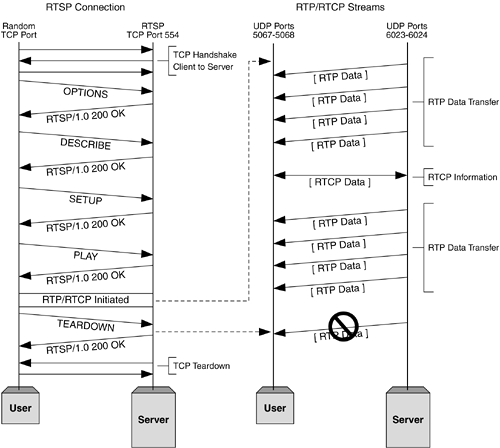
\includegraphics[width=\textwidth]{figures/rtsp_example}
	\caption{Figure of client that interacts with a server. Figure is taken from \url{http://www.informit.com/articles/article.aspx?p=169578&seqNum=3}}
	\label{fig:design:rtsp:example}
\end{figure}

In figure \ref{fig:design:rtsp:example}, an example of a client requesting a stream from a server is shown. As RTSP is run over TCP in the example, a 3-way handshake has to be created before RTSP packets can be sent.
Each of the messages are explained below:
\begin{itemize}
	\item \textbf{OPTIONS} is issued by the client, in order to get information about a stream. The client provides a url to the wanted stream fx. rtsp://example.com/stream.mp4. The server then replies back with "200 OK" if the url exists, and a list of the supported request types such as: Play, pause, teardown etc.
	
	\item \textbf{DESCRIBE} is issued by the client, in order to get a description of the stream. The description is in the SDP format containing information about encoding, bitrate etc. as described in section \ref{sec:design:sdp}.
	
	\item \textbf{SETUP} is issued by the client when the client is ready to configure how the stream should be sent to the client. The client provides two ports in the SETUP request, which denotes the destination port to which the server should send the RTP/RTCP packets.
	
	\item \textbf{PLAY} is issued by the client when the client is ready to get the stream.
When \textbf{PLAY} is received and processed by the server, the server starts to send RTP/RTCP packets to the client to the port provided in the SETUP request.
In order to avoid problems with firewalls between the server and client, the RTP and RTCP packets can be interleaved into the TCP connection created by RTSP.
The \textbf{PLAY} method supports a \textit{range} header, where a range in the stream of the interest can be specified.
The range is used by the client to specify when to see the stream from and to. 
The unit of the range is specified in the \textit{Accept-Ranges} sent in the \textbf{SETUP} method. RFC7826 states, that \ac{NTP} and Absolute Time in ISO8601\footnote{\url{https://www.w3.org/TR/NOTE-datetime}} suporting decimal fractions of seconds, but other units such as bytes\footnote{\url{https://tools.ietf.org/html/rfc7826\#section-18.40}} may be supported as well.
	\item \textbf{TEARDOWN} is issued when the client wants to close the connection. The server will then stop streaming RTP/RTCP, and close the TCP connection.
\end{itemize}

\todo{Mention RECORD + ANNOUNCE}

In RTSP v1.0\citep{RFC2326}, two methods are mentioned which have been removed in RTSP v2.0.
\begin{itemize}
	\item \textbf{RECORD} is issued by the client, when it wants to record part of a live stream. A \textit{Conference} header is present, which relates an existing conference such as RTP multicast session and a RTSP session such that the server knows what to record. A \textit{Range} header similar to \textbf{PLAY} is used to specify a range to be recorded.
	\item \textbf{ANNOUNCE} can be issued by both server and clients in order to inform the opposite part of the properties of a RTP stream. If \textbf{ANNOUNCE} is sent from the client to the server, the method is used to tell the server about a new stream that is available. Other clients can then do a \textbf{DESCRIBE} on the newly created URI in order get a session description. If the method is issued by the server, its because the RTP session has changed and the server is pushing out a new session description.
\end{itemize}


\section{Gstreamer}
Gstreaner is a open source tool available, that implements some of the protocols described in section \ref{sec:design:protocols}.
\todo{Describe gstreamer + pros and cons}
Cons:
 - 64bit timestamp injected
 - Does not handle multicast address assignment
Gstreamer is a pipeline based streaming framework that aims to make it easy to work with streams. Gstreamer is plugin based which allows for adding functionality as needed in applications. The idea of plugins is to create plugins are have a well defined responsibility such as reading a file, encoding, playing etc. The plugins are usually connected in gstreamer pipelines, however then can be used in independent applications. Gstreamer plugins are connected using pads, where each plugin can have a source and sink pad. A source pad can then be connected to the next plugin's sink pad. An example of plugins in a pipelines is showed below:
\begin{figure}
	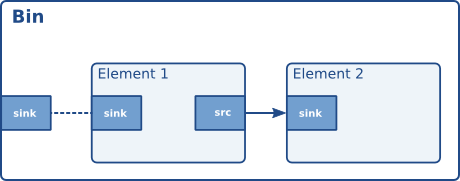
\includegraphics[width=1\textwidth]{figures/bin-element-ghost.png}
\end{figure}

\todo{Describe example figure + rtpbin + rtppay/depay}


\todo{Compare gstreamer with custom impl.}


\subsection{Publisher \& Subscriber}
This section presents the design of the \program{Publisher} and \program{Subscriber} from the extracted requirements from the analysis chapter. The end of this section compares the implementation requirements with the protocols from section \ref{sec:design:protocols}.

\subsubsection{Publisher}

\subsubsection{Subscriber}

Describe given the nature of the stream, that publisher/subscriber most react on incoming data, and else do nothing until a new packet arrives.

This is similar to graphical interfaces, where the input is key press or clicks. This is event driven meaning a callback is invoked when an event is happening.
The subscriber should listen for the following events:
\begin{itemize}
	\item Incoming data packet from the producer
	\item Incoming metadata packet from the producer
	\item Periodically when metadata must be sent
\end{itemize}
\todo{Call "periodically event" for "temporal event"?}

The publisher should listen for the following events:
\begin{itemize}
	\item Incoming packet on stream
	\item Incoming metadata packet on stream
	\item Periodically when metadata must be sent.
\end{itemize}

alternative to event is polling, where the subscriber/publisher polls for data. This would be very CPU consuming and not utilize the functionality provided by the kernel.


\section{Historian}

Comparison of rtpdump(rtptools) and tcpdump+tcpreplay.

% Please add the following required packages to your document preamble:
% \usepackage{graphicx}
\begin{table}[H]
\centering
\resizebox{\textwidth}{!}{%
\begin{tabular}{|l|c|c|}
\hline
\textbf{}       & \textbf{tcpdump/tcpreplay} & \textbf{rtpdump/rtpplay} \\ \hline
Record duration &                            &                          \\ \hline
IPv6 support    & \checkmark  & X                        \\ \hline
Multiple replay &                            &                          \\ \hline
Replay of RTCP  &          \checkmark                 &         X                 \\ \hline
\end{tabular}%
}
\caption{My caption}
\label{my-label}
\end{table}
\section{Stream Topology}

Master vs. nomaster
Cost of wellknown information(Profile + address, port) at all ends.
Describe how streams are put into sessions(RFC about semantics and taxonomics, pros and cons)

